\section{The Large Hadron Collider}
In March 1984, the European Organization for Nuclear Research CERN) and the European Committee for Future Accelerators (ECFA) 
held a workshop in Lausanne entitled "Large Hadron Collider in the LEP Tunnel". 
This is history's first written mention of the Large Hadron Collider (LHC) and the topic under discussion 
was exactly how and where to build a new type of high-energy collider, capable of bringing hadrons
to collide rather than leptons.
The LHC would be housed in a tunnel which, at the time, was under excavation to host the Large Electron-Positron Collider (LEP) designed to collide leptons with center-of-mass-energies up to around 200 GeV.
LEP was a circular collider with a circumference of 27 km and the tunnel hosting it was located roughly 100 meters underground on the border between France and Switzerland, at the outskirts of Geneva. 
The justification for building a machine like the LHC, was that once LEP got to maximum reach, a new and more powerful collider would be needed in its place in order to probe higher energies.
While collisions of electrons with positrons provided exceptionally clean and precise measurements due to them being point particles,
 their lightness prevent them from being accelerated to higher energies. Collisions of hadrons, however, would allow for center-of-mass energies two orders of magnitude higher than that of LEP. Therefore, after running a while at two times the W mass (160 GeV) and reaching a maximum center-of-mass energy of 209 GeV, LEP was dismantled in 2000 in order to make room for the LHC.
 
The Large Hadron Collider started up in September 2008 and, while having the same 27-kilometer radius as the LEP collider, is capable of accelerating protons up to a center-of-mass energy of around 14 TeV, 70 times that of LEP. The accelerator consists of two oppositely going proton beams, isolated from each other and under ultrahigh vacuum, which are accelerated up to speeds close to that of the speed of light through radiofrequency (RF) cavities, before being brought to collide at four different interaction points along the ring.
These four collision points correspond to the location of the four LHC particle detectors; ATLAS, CMS, LHCb and ALICE.
While ATLAS and CMS are general-purpose detectors built in order to study a large range of different physics processes, 
LHCb and ALICE are built for dedicated purposes; LHCb for b-physics processes and ALICE for heavy ion collision.
A protons journey from gas to one of the LHC collision points is as follows: First, hydrogen nuclei are extracted from a small tank of compressed hydrogen gas and stripped of their electrons. The remaining protons are then

\begin{figure}[h]
    \centering
    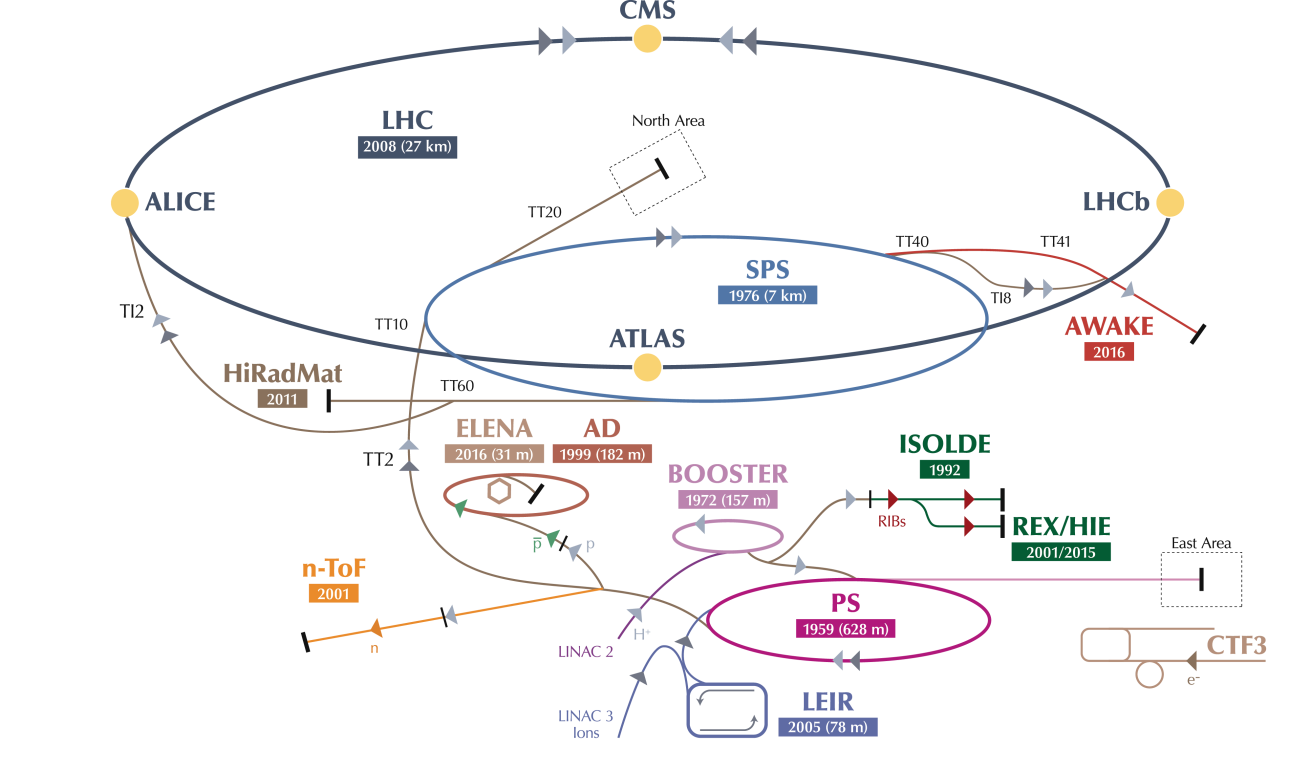
\includegraphics[width=0.90\textwidth]{figures/cms/LHC.png}
    \caption{The Large Hadron Collider accelerator complex. The four collision points along the ring correspond to the location of the LHC particle detectors CMS, LHCb, ATLAS and ALICE~\cite{LHC}.}
    \label{fig:cms:LHC}
\end{figure}


\section{The CMS detector}
\subsection{Pixel detector and strip tracker}
\subsection{Electromagnetic calorimeter}
\subsection{Hadronic calorimeter}
\subsection{Muon chambers}
\section{Trigger system: From collision to disk}
